\begin{minipage}{\textwidth}
    \setlength{\parindent}{2em}
    Following the analysis of the system requirements, this section outlines the \textbf{database tables supporting the modules and features under my responsibility}. It provides both a high-level overview and detailed descriptions of the entities, their attributes, and their relationships.
\end{minipage}


\subsubsection{Extracted database tables}
\noindent
\begin{minipage}{\textwidth}
    \setlength{\parindent}{2em}
    This part illustrated the \textbf{high-level overview of the extracted database tables for modules and features under my responsibility} through the Entity-Relationship Diagram (ERD). The ERD visually represents the core entities, their attributes, and the relationships between them.
\end{minipage}
\begin{figure}[H]
    \centering
    % 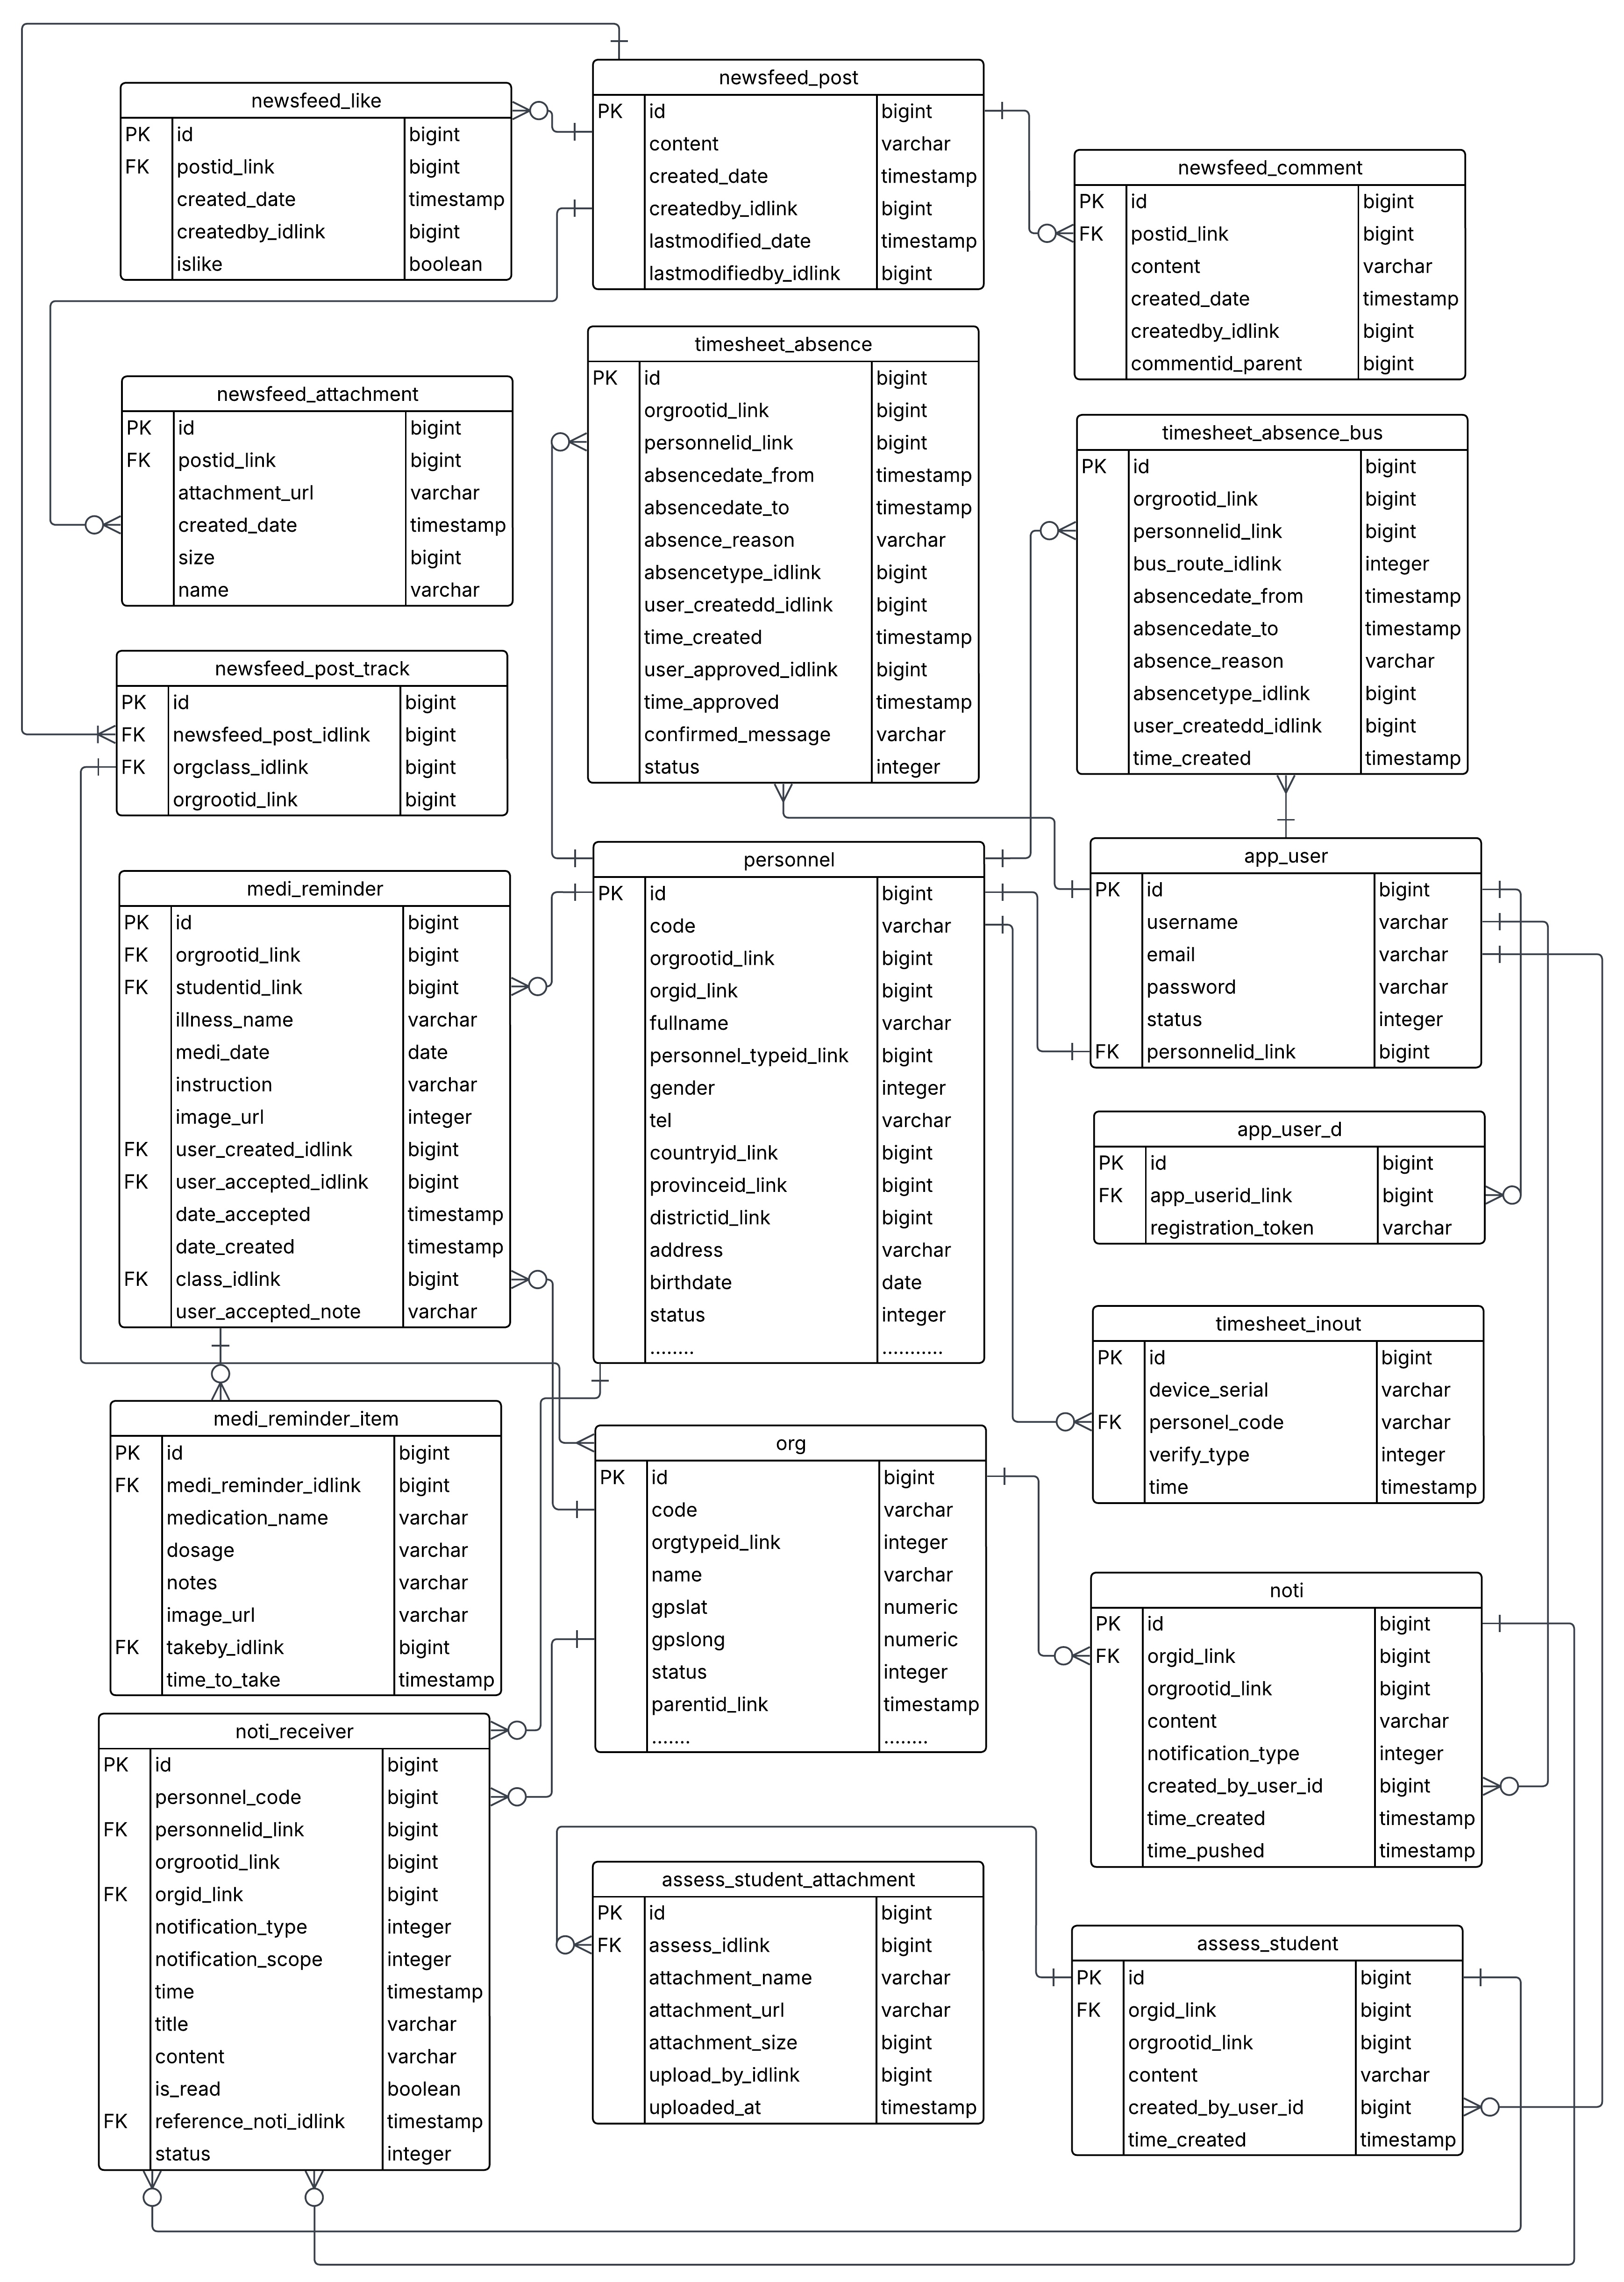
\includegraphics[width=1.05\textwidth]{images/database_erd.png}
    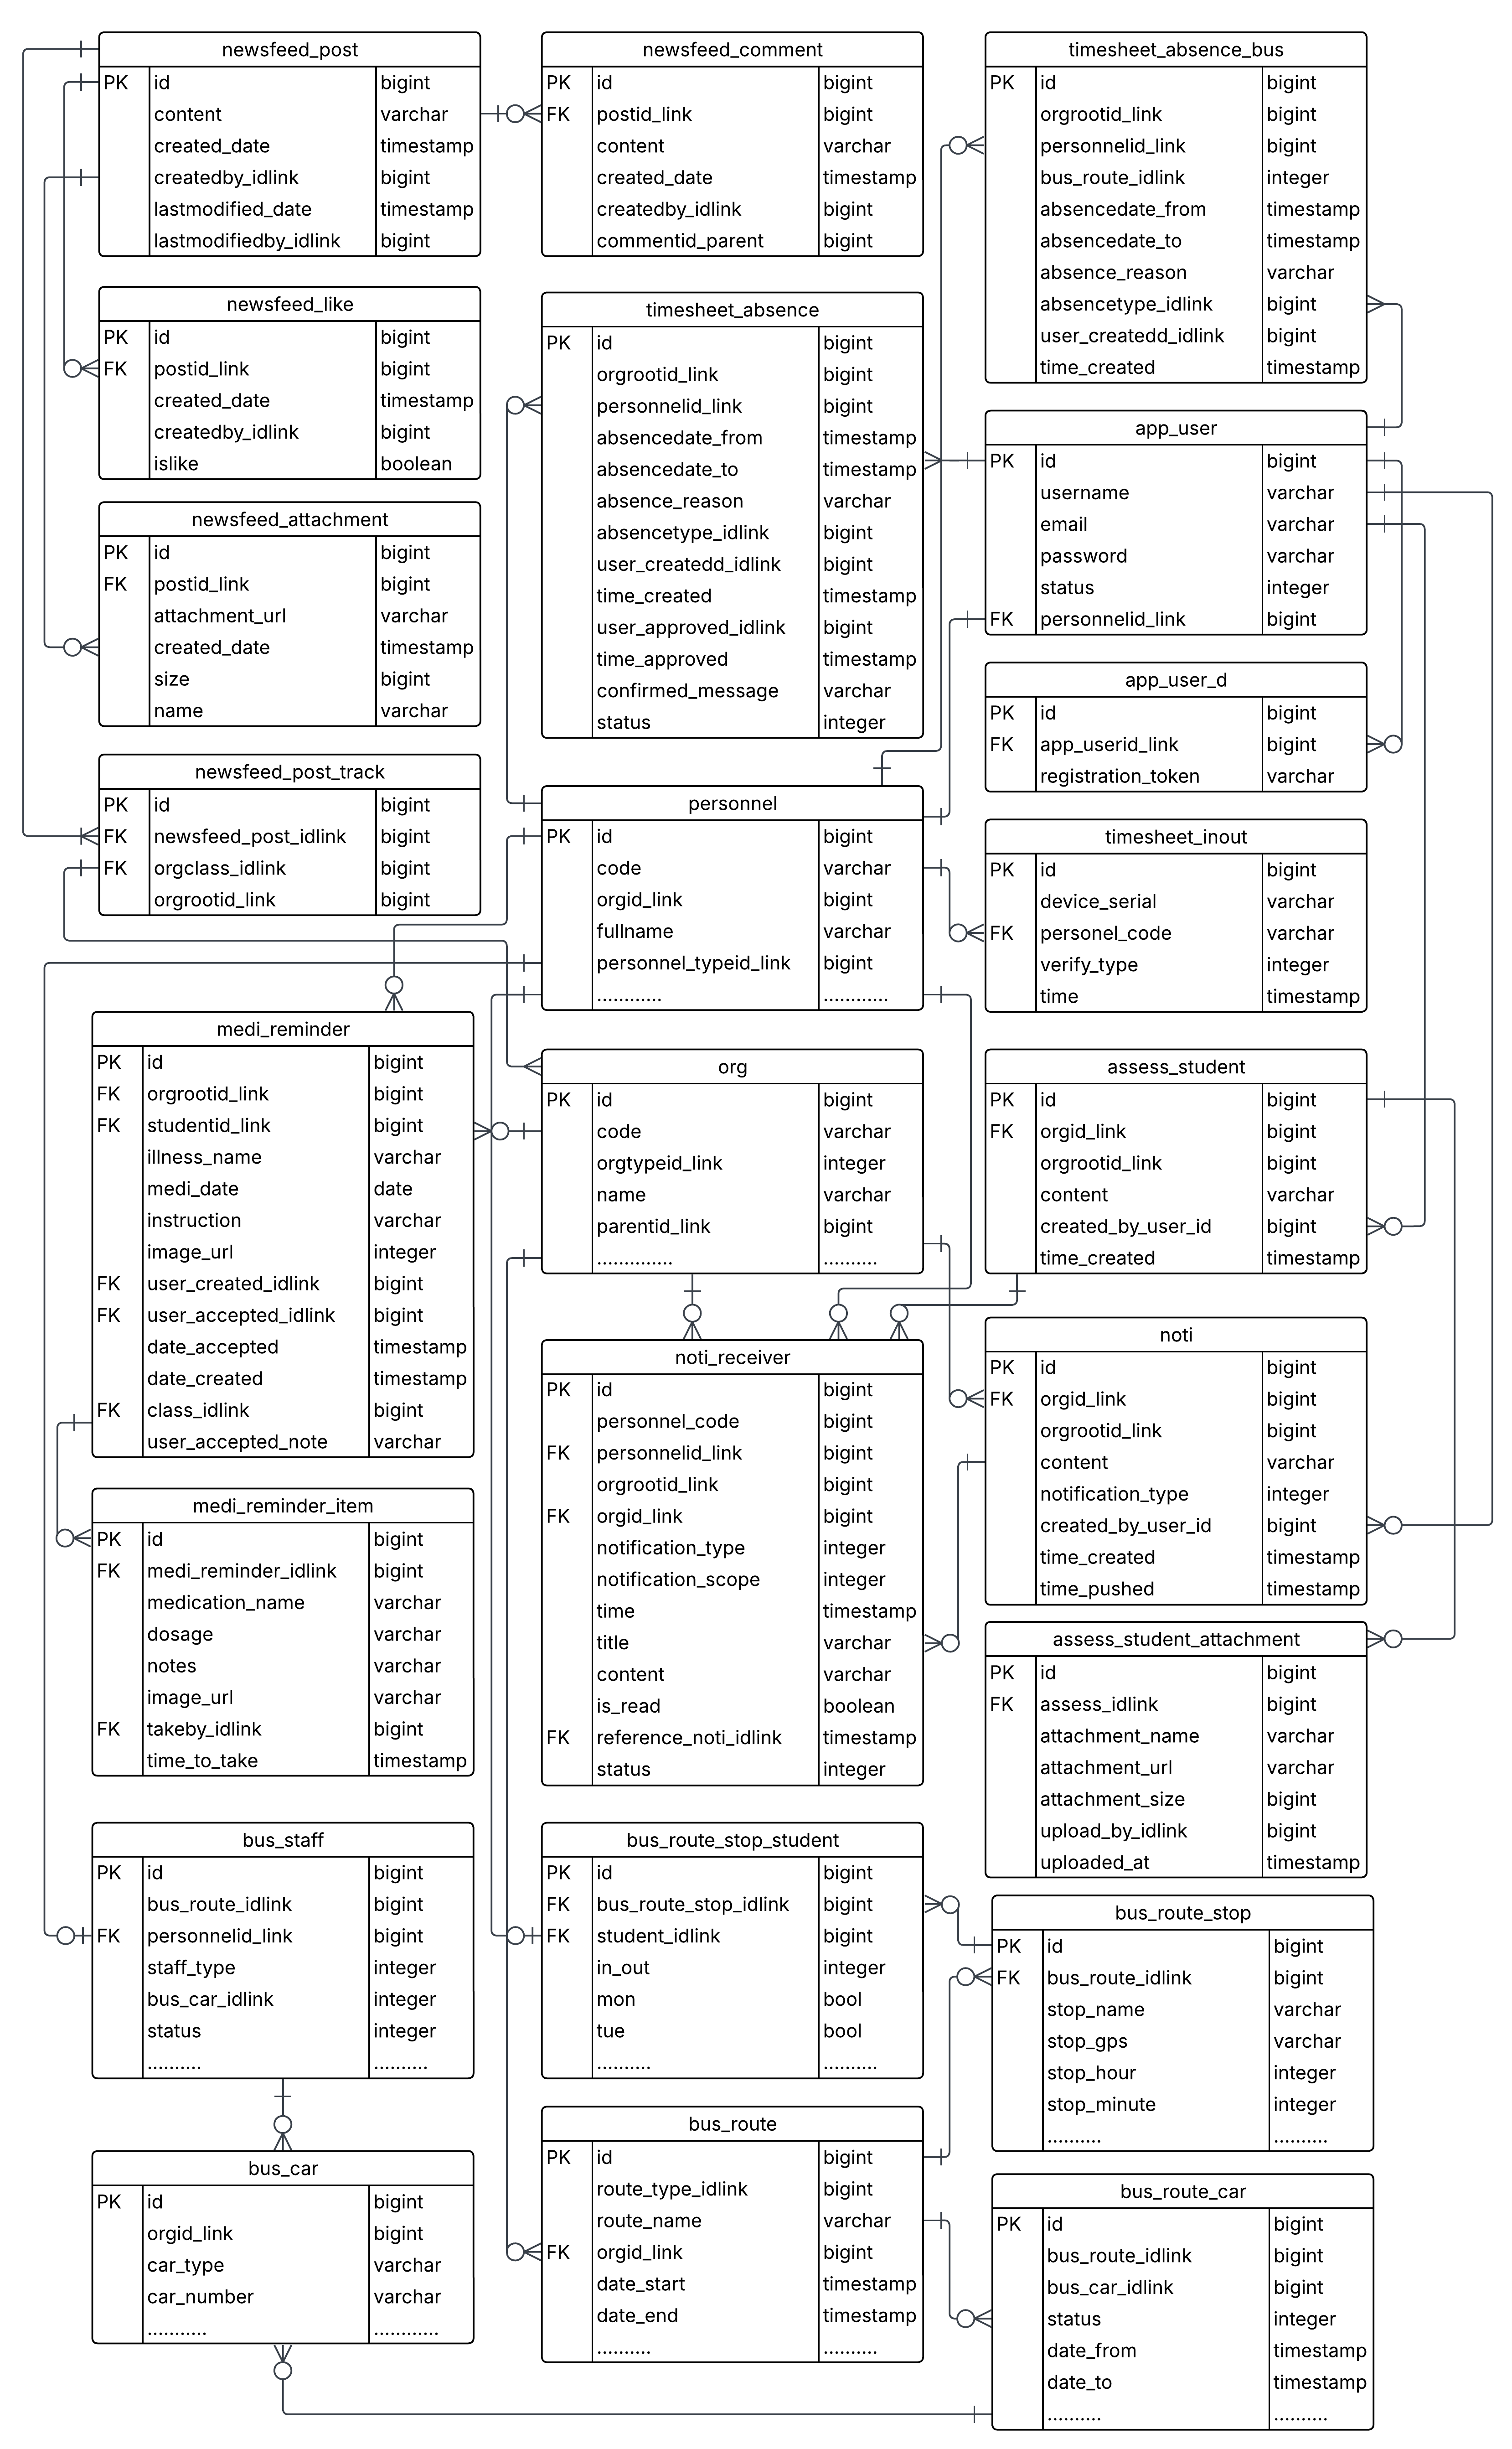
\includegraphics[width=1\textwidth]{images/image.png}
    \caption{Extracted database tables.}
    \label{fig:database_erd}
\end{figure}

\subsubsection{Database Design Description}
\noindent
\begin{minipage}{\textwidth}
    \setlength{\parindent}{2em}
    This section explain the \textbf{Extracted database tables} illustrated in \textbf{\autoref{fig:database_erd}} that related to the \textbf{features and modules assigned to me} in this project. Below is a detailed description of each entity and the relationships between them.
    % In this section, we will explain the Entity-Relationship Diagram (ERD) illustrated in \textbf{\autoref{fig:database_erd}} by describing each entity and its attributes, the relationships and cardinalities between entities, and how this design supports the system requirements.
\end{minipage}
\vspace{-0.8em}
\begin{itemize}[itemsep=-0.1cm]
    \item \textbf{personnel}: The table stores detailed information about both employees and students, which can be identified using the personnel\_typeid\_link attribute. It includes basic personal details (name, gender, birth date, contact, status) along with additional data specific to students and employees. This design ensures efficient management of personal information.
    \item \textbf{org}: The org table stores information about all organizational units (schools, departments, classes, etc) and uses the parentid\_link attribute to maintain a hierarchical structure.
    \item \textbf{app\_user}: This table stores user login credentials and controls access to the system. For security purposes, all passwords are encrypted using the Bcrypt hashing algorithm.
    \item \textbf{app\_user\_d}: The table manages mobile device access by linking each device token to a user account. These tokens are then used to send notifications.
    \item \textbf{timesheet\_inout}: The table is used to record raw attendance data. It tracks which device was used (device\_serial), the verification method: face recognition, fingerprint, or manual entry by a teacher (verify\_type), and the time when attendance was recorded.
    \item \textbf{timesheet\_absence}: Stores leave requests for employees and students. It records the absence dates, reason, leave type, and tracks the complete approval process including who submitted it, when it was created, who approved it, and approval time.
    \item \textbf{timesheet\_absence\_bus}: The table is used to track bus leave requests when students request time off from bus service, ensuring coordination between attendance and transportation management.
    \item \textbf{newsfeed\_post}: The main table for storing newsfeed content. Each post can be associated with multiple related entities, including newsfeed likes, comments, and attachments, enabling scalability.
    \item \textbf{newsfeed\_attachment}: The table manages attachments associated with newsfeed posts using URLs. It stores metadata like file name, size, and creation time, while the actual files are stored on the server and referenced by URLs.
    \item \textbf{newsfeed\_like}: The table manages user reactions to newsfeed posts, tracking which users have interacted with specific posts.
    \item \textbf{newsfeed\_comment}: The table manages user comments on newsfeed posts. It tracks who commented, the content, and timestamp while supporting hierarchical reply structures through the commentid\_parent field.
    \item \textbf{medi\_reminder}: The table stores the medicine reminders for students. It captures illness details, medication dates, treatment instructions, and tracks who created the reminder and which teacher confirmed it.
    \item \textbf{medi\_reminder\_item}: The table stores individual medicine details within each reminder request. These records maintain a direct relationship with their corresponding medication reminders through the medi\_reminder\_idlink.
    \item \textbf{assess\_student}: The assess\_student manages assessments for individual or multiple students.
    \item \textbf{assess\_student\_attachment}: The table manages file attachments associated with assessments using URLs. It stores metadata like file name, size, and creation time.
    \item \textbf{noti}: The table stores notifications to be pushed to users. Each record contains content, title, scope (whole organization, school, or class level), and type (attendance, leave requests, medicine reminders, etc.)
    \item \textbf{noti\_receiver}: The table tracks notifications or assessments sent to individual users. It records who received it, when it was sent, read status, and delivery status.
    \item \textbf{bus\_route}: The table is designed to store and manage information about bus routes. Its primary purpose is to track details such as route names, assigned vehicles, drivers, managers, and operational schedules, ensuring efficient organization and monitoring of bus routes.
    \item \textbf{bus\_route\_stop}: The table designed to store individual pickup and drop-off points  within a bus route. It define the sequential priority, timing, and location of stops, ensuring accurate scheduling and reliable navigation for both transportation staff and students.
    \item \textbf{bus\_route\_stop\_student}: The table links students to specific bus routes and stops, helping the system track assignments and improve bus operation efficiency and safety.
    \item \textbf{bus\_route\_staff}: The table assigns transportation staff (drivers, managers) to bus routes, allowing flexible allocation of drivers and managers to different routes as needed.
    \item \textbf{bus\_route\_car}: This table links buses to routes over time, allowing flexible assignments and preventing scheduling conflicts across the transportation network.
    \item \textbf{bus\_car}: The table stores detailed information about all school buses including vehicle type, license plate, description, and seating capacity. This centralized registry enables efficient assignment of specific buses to designated routes, ensuring optimal fleet utilization and proper matching of vehicle capacity to route requirements.
\end{itemize}